\documentclass[addpoints,spanish, 12pt,a4paper]{exam}
%\documentclass[answers, spanish, 12pt,a4paper]{exam}
   \printanswers
\pointpoints{punto}{puntos}
\hpword{Puntos:}
\vpword{Puntos:}
\htword{Total}
\vtword{Total}
\hsword{Resultado:}
\hqword{Ejercicio:}
\vqword{Ejercicio:}

\usepackage[utf8]{inputenc}
\usepackage[spanish]{babel}
\usepackage{eurosym}
%\usepackage[spanish,es-lcroman, es-tabla, es-noshorthands]{babel}
\usepackage{pgf,tikz}


\usepackage[margin=1in]{geometry}
\usepackage{amsmath,amssymb}
\usepackage{multicol}
\usepackage{yhmath}

\pointsinrightmargin % Para poner las puntuaciones a la derecha. Se puede cambiar. Si se comenta, sale a la izquierda.
\extrawidth{-2.4cm} %Un poquito más de margen por si ponemos textos largos.
\marginpointname{ \emph{\points}}

\usepackage{graphicx}

\graphicspath{{../img/}} 

\newcommand{\class}{4º Académicas}
\newcommand{\examdate}{\today}
\newcommand{\examnum}{Global 3ª evaluación}
\newcommand{\tipo}{A}


\newcommand{\timelimit}{50 minutos}

\renewcommand{\solutiontitle}{\noindent\textbf{Solución:}\enspace}


\pagestyle{head}
\firstpageheader{
\includegraphics[width=0.2\columnwidth]{header_left}}{\textbf{Departamento de Matemáticas\linebreak \class}\linebreak \examnum}{
\includegraphics[width=0.1\columnwidth]{header_right}}
\runningheader{\class}{\examnum}{Página \thepage\ of \numpages}
\runningheadrule

\DeclareUnicodeCharacter{2212}{-}
\begin{document}

\noindent
\begin{tabular*}{\textwidth}{l @{\extracolsep{\fill}} r @{\extracolsep{6pt}} }
\textbf{Nombre:} \makebox[3.5in]{\hrulefill} & \textbf{Fecha:}\makebox[1in]{\hrulefill} \\
 & \\
\textbf{Tiempo: \timelimit} & Tipo: \tipo 
\end{tabular*}
\rule[2ex]{\textwidth}{2pt}
Esta prueba tiene \numquestions\ ejercicios. La puntuación máxima es de \numpoints. 
La nota final de la prueba será la parte proporcional de la puntuación obtenida sobre la puntuación máxima. 

\begin{center}


\addpoints
 %\gradetable[h][questions]
	\pointtable[h][questions]
\end{center}

\noindent
\rule[2ex]{\textwidth}{2pt}

\begin{questions}


% \question[1] 
% \begin{solution} \end{solution}
% \addpoints

% \question[1] 
% \begin{solution} \end{solution}
% \addpoints


\question Calcula $x$ e $y$ para que los vectores $\overrightarrow{u}$ y $\overrightarrow{v}$ sean perpendiculares a $\overrightarrow{w}$:\begin{parts} \part[1] Siendo $\overrightarrow{u}\left( x, \  2\right), \ \overrightarrow{v}\left( -6, \  y\right)y \ \overrightarrow{w}\left( 2, \  -3\right)$ \begin{solution} $x=3\ \land $$\ y=-4$\end{solution} \part[1] Siendo $\overrightarrow{u}\left( x, \  4\right), \ \overrightarrow{v}\left( -10, \  y\right)y \ \overrightarrow{w}\left( 4, \  5\right)$ \begin{solution} $x=-5\ \land $$\ y=8$\end{solution} \end{parts}

\question Calcula el vector que une los puntos $P$ y $Q$ y su módulo.\begin{parts} \part[1] Siendo $P\left( -2, \  0\right)$ y $Q\left( 12, \  0\right)$\begin{solution} $dist(P,Q)=|Point2D\left(14, 0\right)|=14$\end{solution} \part[1] Siendo $P\left( -1, \  1\right)$ y $Q\left( 3, \  1\right)$\begin{solution} $dist(P,Q)=|Point2D\left(4, 0\right)|=4$\end{solution} \part[1] Siendo $P\left( -2, \  2\right)$ y $Q\left( 3, \  -4\right)$\begin{solution} $dist(P,Q)=|Point2D\left(5, -6\right)|=\sqrt{61}$\end{solution} \end{parts} 

\question Sean A, B, C y D los vértices consecutivos del paralelogramos ABCD. Calcula analíticamente su perímetro: \begin{parts} \part[1] Sabiendo que $A$, $B$ y $C$ son respectivamente: $\left( 3, \  0\right) $, $\left( 5, \  0\right) $, $\left( 5, \  2\right)$\begin{solution} $\overrightarrow{AB} = \overrightarrow{DC} \to Point2D\left(2, 0\right) = Point2D\left(5 - x, 2 - y\right) \to D\left( 3, \  2\right)\to dis(AB)=2\  dis(BC)=2\to 8\to 8$\end{solution} \part[1] Sabiendo que $A$, $B$ y $C$ son respectivamente: $\left( 3, \  -3\right) $, $\left( 6, \  -1\right) $, $\left( 5, \  4\right)$\begin{solution} $\overrightarrow{AB} = \overrightarrow{DC} \to Point2D\left(3, 2\right) = Point2D\left(5 - x, 4 - y\right) \to D\left( 2, \  2\right)\to dis(AB)=\sqrt{13}\  dis(BC)=\sqrt{26}\to 2 \sqrt{13} + 2 \sqrt{26}\to 17.4$\end{solution} \part[1] Sabiendo que $A$, $B$ y $C$ son respectivamente: $\left( -1, \  -2\right) $, $\left( 6, \  -1\right) $, $\left( 5, \  4\right)$\begin{solution} $\overrightarrow{AB} = \overrightarrow{DC} \to Point2D\left(7, 1\right) = Point2D\left(5 - x, 4 - y\right) \to D\left( -2, \  3\right)\to dis(AB)=5 \sqrt{2}\  dis(BC)=\sqrt{26}\to 2 \sqrt{26} + 10 \sqrt{2}\to 24.34$\end{solution} \end{parts}

\question Sean A, B, C y D los vértices consecutivos del paralelogramos ABCD. Calcula analíticamente su centro: \begin{parts} \part[1] Sabiendo que $A$, $B$ y $C$ son respectivamente: $\left( 3, \  0\right) $, $\left( 5, \  0\right) $, $\left( 5, \  2\right)$\begin{solution} $\overrightarrow{AB} = \overrightarrow{DC} \to Point2D\left(2, 0\right) = Point2D\left(5 - x, 2 - y\right) \to D\left( 3, \  2\right)\to M_{AC}=Point2D\left(4, 1\right)$\end{solution} \part[1] Sabiendo que $A$, $B$ y $C$ son respectivamente: $\left( 3, \  -3\right) $, $\left( 6, \  -1\right) $, $\left( 5, \  4\right)$\begin{solution} $\overrightarrow{AB} = \overrightarrow{DC} \to Point2D\left(3, 2\right) = Point2D\left(5 - x, 4 - y\right) \to D\left( 2, \  2\right)\to M_{AC}=Point2D\left(4, \dfrac{1}{2}\right)$\end{solution} \part[1] Sabiendo que $A$, $B$ y $C$ son respectivamente: $\left( -1, \  -2\right) $, $\left( 6, \  -1\right) $, $\left( 5, \  4\right)$\begin{solution} $\overrightarrow{AB} = \overrightarrow{DC} \to Point2D\left(7, 1\right) = Point2D\left(5 - x, 4 - y\right) \to D\left( -2, \  3\right)\to M_{AC}=Point2D\left(2, 1\right)$\end{solution} \end{parts} 



\question Escribe las ecuaciones vectorial, paramétricas, en forma continua y explícita de la recta que:\begin{parts} \part[1] Pasa por los punto $P\left( -3, \  -1\right)$ y $Q\left( 3, \  2\right)$\begin{solution} Solución orientativa: $Point2D\left(x, y\right) = Point2D\left(6 t - 3, 3 t - 1\right) \to - 3 x + 6 y - 3 = 0 \to y = \dfrac{x}{2} + \dfrac{1}{2}$\end{solution} \part[1] Pasa por los punto $P\left( 1, \  -2\right)$ y $Q\left( 4, \  4\right)$\begin{solution} Solución orientativa: $Point2D\left(x, y\right) = Point2D\left(3 t + 1, 6 t - 2\right) \to - 6 x + 3 y + 12 = 0 \to y = 2 x - 4$\end{solution} \part[1] Pasa por los punto $P\left( 7, \  -2\right)$ y $Q\left( 4, \  4\right)$\begin{solution} Solución orientativa: $Point2D\left(x, y\right) = Point2D\left(7 - 3 t, 6 t - 2\right) \to - 6 x - 3 y + 36 = 0 \to y = 12 - 2 x$\end{solution} \end{parts} 


\question Calcula la recta $s$ que:\begin{parts} \part[1] Pasa por $P\left( -1, \  2\right)$ y es perpendicular a la recta que pasa por $Q\left( 3, \  2\right)$ y tiene como vector director $\overrightarrow{d_r}\left( -2, \  1\right)$\begin{solution} $s\equiv 2 x - y + 4 = 0$\end{solution} \part[1] Pasa por $P\left( 2, \  -4\right)$ y es perpendicular a la recta que pasa por $Q\left( 1, \  1\right)$ y tiene como vector director $\overrightarrow{d_r}\left( 3, \  1\right)$\begin{solution} $s\equiv - 3 x - y + 2 = 0$\end{solution} \end{parts} 


\question Responde a las siguientes cuestiones:\begin{parts} \part[3] Las calificaciones de un grupo de 30 alumnos han sido: 9 6 5 1 5 7 9 10 7 5 1 2 5 7 6 4 6 8 8 6 4 4 6 5 3 5 7 7 8 7. \begin{itemize} \item Realiza una tabla de frecuencias \item Calcular los siguientes parámetros de centralización: media, mediana y moda \item Calcular los siguientes parámetros de posición: P70, Q1, Q3 \item Calcular los siguientes parámetros de dispersión: varianza, desviación típica y coeficiente de variación \item Realiza un diagrama de caja y bigote. \end{itemize}\begin{solution} $\begin{tabular}{rrrrrrr}
\hline
   $x_i$ &   $f_i$ &   $F_i$ &    $\%_i$ &   $\%A_i$ &   $x_if_i$ &   $x^2_if_i$ \\
\hline
       1 &       2 &       2 &   6.66667 &   6.66667 &          2 &            2 \\
       2 &       1 &       3 &   3.33333 &  10       &          2 &            4 \\
       3 &       1 &       4 &   3.33333 &  13.3333  &          3 &            9 \\
       4 &       3 &       7 &  10       &  23.3333  &         12 &           48 \\
       5 &       6 &      13 &  20       &  43.3333  &         30 &          150 \\
       6 &       5 &      18 &  16.6667  &  60       &         30 &          180 \\
       7 &       6 &      24 &  20       &  80       &         42 &          294 \\
       8 &       3 &      27 &  10       &  90       &         24 &          192 \\
       9 &       2 &      29 &   6.66667 &  96.6667  &         18 &          162 \\
      10 &       1 &      30 &   3.33333 & 100       &         10 &          100 \\
     nan &      30 &     nan & 100       & nan       &        173 &         1141 \\
\hline
\end{tabular}$\\ 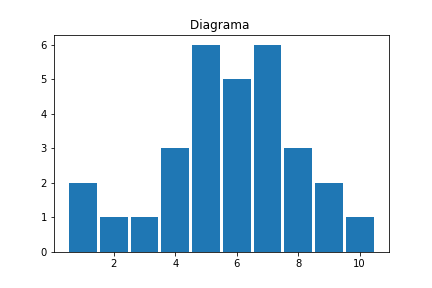
\includegraphics[width=0.7\columnwidth]{diagrama_ex0} \\ $\left\{ Me : 6.0, \  Mo : \left( [5], \  [6]\right), \  media : 5.77\right\}$ \\$\left\{ P70 : 7.0, \  Q1 : 5.0, \  Q3 : 7.0\right\}$ \\$\left\{ C.V : 0.38, \  desv.tip : 2.19, \  rango : 9, \  var : 4.78\right\}$\\ 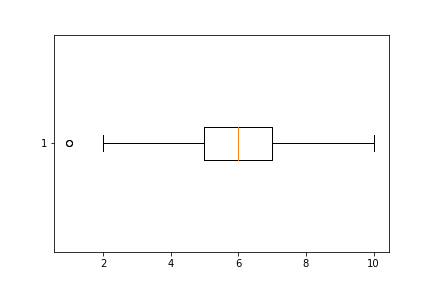
\includegraphics[width=0.7\columnwidth]{caja_ex0}\end{solution} \part[3] Las calificaciones de un grupo de 30 alumnos han sido: 3 2 2 4 6 6 6 7 7 7 2 5 5 5 4 7 8 8 8 8 4 4 7 7 8 9 9 9 10 10. \begin{itemize} \item Realiza una tabla de frecuencias \item Calcular los siguientes parámetros de centralización: media, mediana y moda \item Calcular los siguientes parámetros de posición: P70, Q1, Q3 \item Calcular los siguientes parámetros de dispersión: varianza, desviación típica y coeficiente de variación \item Realiza un diagrama de caja y bigote. \end{itemize}\begin{solution} $\begin{tabular}{rrrrrrr}
\hline
   $x_i$ &   $f_i$ &   $F_i$ &    $\%_i$ &   $\%A_i$ &   $x_if_i$ &   $x^2_if_i$ \\
\hline
       2 &       3 &       3 &  10       &   10      &          6 &           12 \\
       3 &       1 &       4 &   3.33333 &   13.3333 &          3 &            9 \\
       4 &       4 &       8 &  13.3333  &   26.6667 &         16 &           64 \\
       5 &       3 &      11 &  10       &   36.6667 &         15 &           75 \\
       6 &       3 &      14 &  10       &   46.6667 &         18 &          108 \\
       7 &       6 &      20 &  20       &   66.6667 &         42 &          294 \\
       8 &       5 &      25 &  16.6667  &   83.3333 &         40 &          320 \\
       9 &       3 &      28 &  10       &   93.3333 &         27 &          243 \\
      10 &       2 &      30 &   6.66667 &  100      &         20 &          200 \\
     nan &      30 &     nan & 100       &  nan      &        187 &         1325 \\
\hline
\end{tabular}$\\ 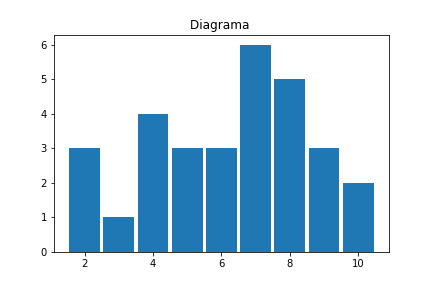
\includegraphics[width=0.7\columnwidth]{diagrama_ex1} \\ $\left\{ Me : 7.0, \  Mo : \left( [7], \  [6]\right), \  media : 6.23\right\}$ \\$\left\{ P70 : 8.0, \  Q1 : 4.25, \  Q3 : 8.0\right\}$ \\$\left\{ C.V : 0.37, \  desv.tip : 2.3, \  rango : 8, \  var : 5.31\right\}$\\ 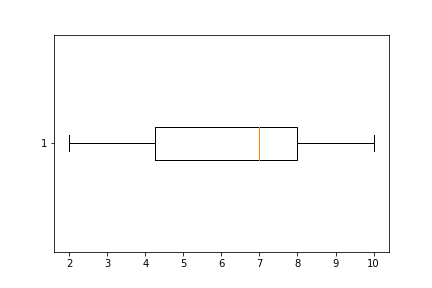
\includegraphics[width=0.7\columnwidth]{caja_ex1}\end{solution} \end{parts} 

\question Se tiene una cometa volando en el aire y anclada al suelo con el hilo. Calcula el ángulo que forma el hilo de la cometa con el suelo:\begin{parts} \part[1] Sabiendo que la longitud del hilo es de 16m. y la cometa se encuentra a 8 m. de alturala hipotenusa mide 16 y un cateto 8 cm.\begin{solution} Los lados del triángulo miden: $8$, $13.86$, $16$ cm. Y los ángulos: $30.0$, $60.0$, $90$ º\end{solution} \part[1] Sabiendo que la longitud del hilo es de 24m. y la cometa se encuentra a 12 m. de alturala hipotenusa mide 24 y un cateto 12 cm.\begin{solution} Los lados del triángulo miden: $12$, $20.78$, $24$ cm. Y los ángulos: $30.0$, $60.0$, $90$ º\end{solution} \end{parts}

\question Resuelve las siguientes ecuaciones (solo las soluciones que estén entre 0 y 360 grados)\begin{parts} \part[1] $\dfrac{1}{2}+\sin{x}=1$\begin{solution} $x=30^{\circ}, x=150^{\circ}$\end{solution} \part[1] $\cos{x}-\dfrac{1}{4}=\dfrac{1}{4}$\begin{solution} $x=60^{\circ}, x=300^{\circ}$\end{solution} \end{parts} 


\addpoints

\end{questions}

\end{document}
\grid
